% 图 2
\documentclass[tikz,border=4pt]{standalone}
\usepackage{amsmath,bm}
\usetikzlibrary{arrows.meta,calc}

\begin{document}
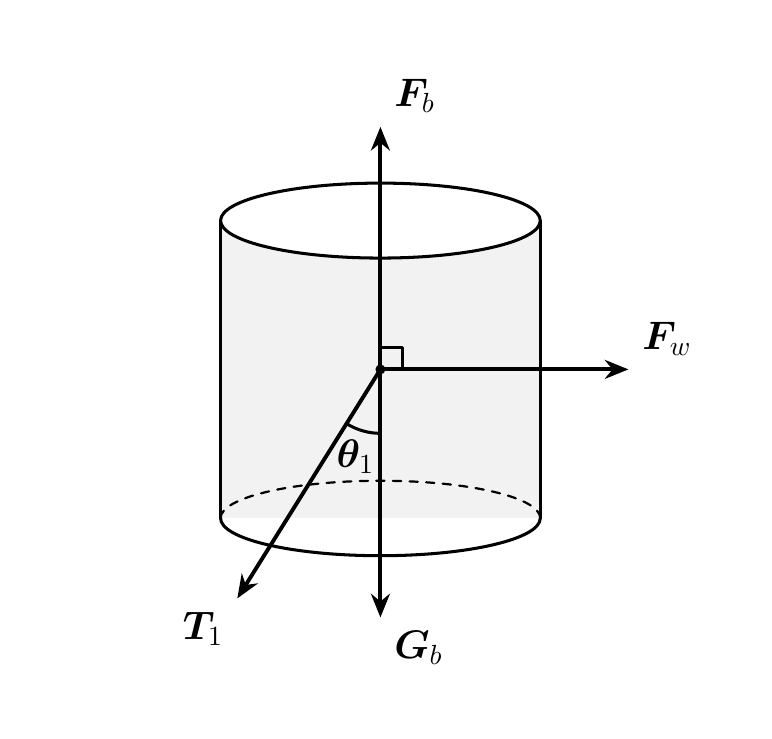
\begin{tikzpicture}[
  x=1.4cm,
  y=1.4cm,
  line cap=round,
  line join=round,
  cylinder/.style={
    draw=black,
    line width=1.1pt
  },
  force/.style={
    draw=black,
    line width=1.4pt,
    -{Stealth[length=3mm,width=2.4mm]}
  },
  anglemark/.style={
    draw=black,
    line width=1.1pt
  },
  label/.style={
    font=\Large\bfseries
  }
]

  % 可调参数
  \def\R{1.45}
  \def\ry{0.34}
  \def\ytop{1.35}
  \def\ybot{-1.35}
  \def\thetaone{32}

  % 圆柱侧面填充
  \fill[black!5]
    (-\R,\ybot) rectangle (\R,\ytop);

  % 上端面
  \filldraw[cylinder,fill=white]
    (0,\ytop)
    ellipse[
      x radius=\R,
      y radius=\ry
    ];

  % 左右母线
  \draw[cylinder]
    (-\R,\ybot) -- (-\R,\ytop);

  \draw[cylinder]
    (\R,\ybot) -- (\R,\ytop);

  % 下端面前半部分
  \draw[cylinder]
    (-\R,\ybot)
    arc[
      start angle=180,
      end angle=360,
      x radius=\R,
      y radius=\ry
    ];

  % 下端面后半部分
  \draw[
    draw=black,
    dashed,
    line width=0.8pt
  ]
    (\R,\ybot)
    arc[
      start angle=0,
      end angle=180,
      x radius=\R,
      y radius=\ry
    ];

  % 共同作用点
  \coordinate (O) at (0,0);
  \fill (O) circle[radius=1.8pt];

  % F_b
  \draw[force]
    (O) -- (0,2.20)
    node[label,above right=1pt] {$\bm{F}_b$};

  % F_w
  \draw[force]
    (O) -- (2.25,0)
    node[label,above right=1pt] {$\bm{F}_w$};

  % G_b
  \draw[force]
    (O) -- (0,-2.25)
    node[label,below right=1pt] {$\bm{G}_b$};

  % T_1
  \draw[force]
    (O) --
    (
      {-2.45*sin(\thetaone)},
      {-2.45*cos(\thetaone)}
    )
    node[label,below left=1pt] {$\bm{T}_1$};

  % theta_1 圆弧
  \draw[anglemark]
    ($(O)+(-90:0.58)$)
    arc[
      start angle=-90,
      end angle={-90-\thetaone},
      radius=0.58
    ];

  % theta_1 标注
  \node[label] at
    (
      {-0.82*sin(\thetaone/2)},
      {-0.82*cos(\thetaone/2)}
    )
    {$\bm{\theta}_1$};

  % 直角标记
  \draw[
    draw=black,
    line width=1pt
  ]
    (0,0.20)
    -- (0.20,0.20)
    -- (0.20,0);

  \path[use as bounding box]
    (-3.2,-3.1) rectangle (3.3,3.1);

\end{tikzpicture}
\end{document}